% in-line formeln
abdcdasd $\sum_{n=1}^{k}\rho_n$
% formeln als Block
\begin{align*} 
	\sum_{n=1}^{k}\rho_n
\end{align*}

%sehen unterschiedlich aus

\subsection{Thema 1}
	absasfasdf
\subsection{Thema 2}
	
	\begin{itemize}
		\item Halbleiter1
		\begin{enumerate}
			\item Montag
			\item Montag
			\item Montag
			\item Montag
		\end{enumerate}
		\item Halbleiter2
	\end{itemize}
	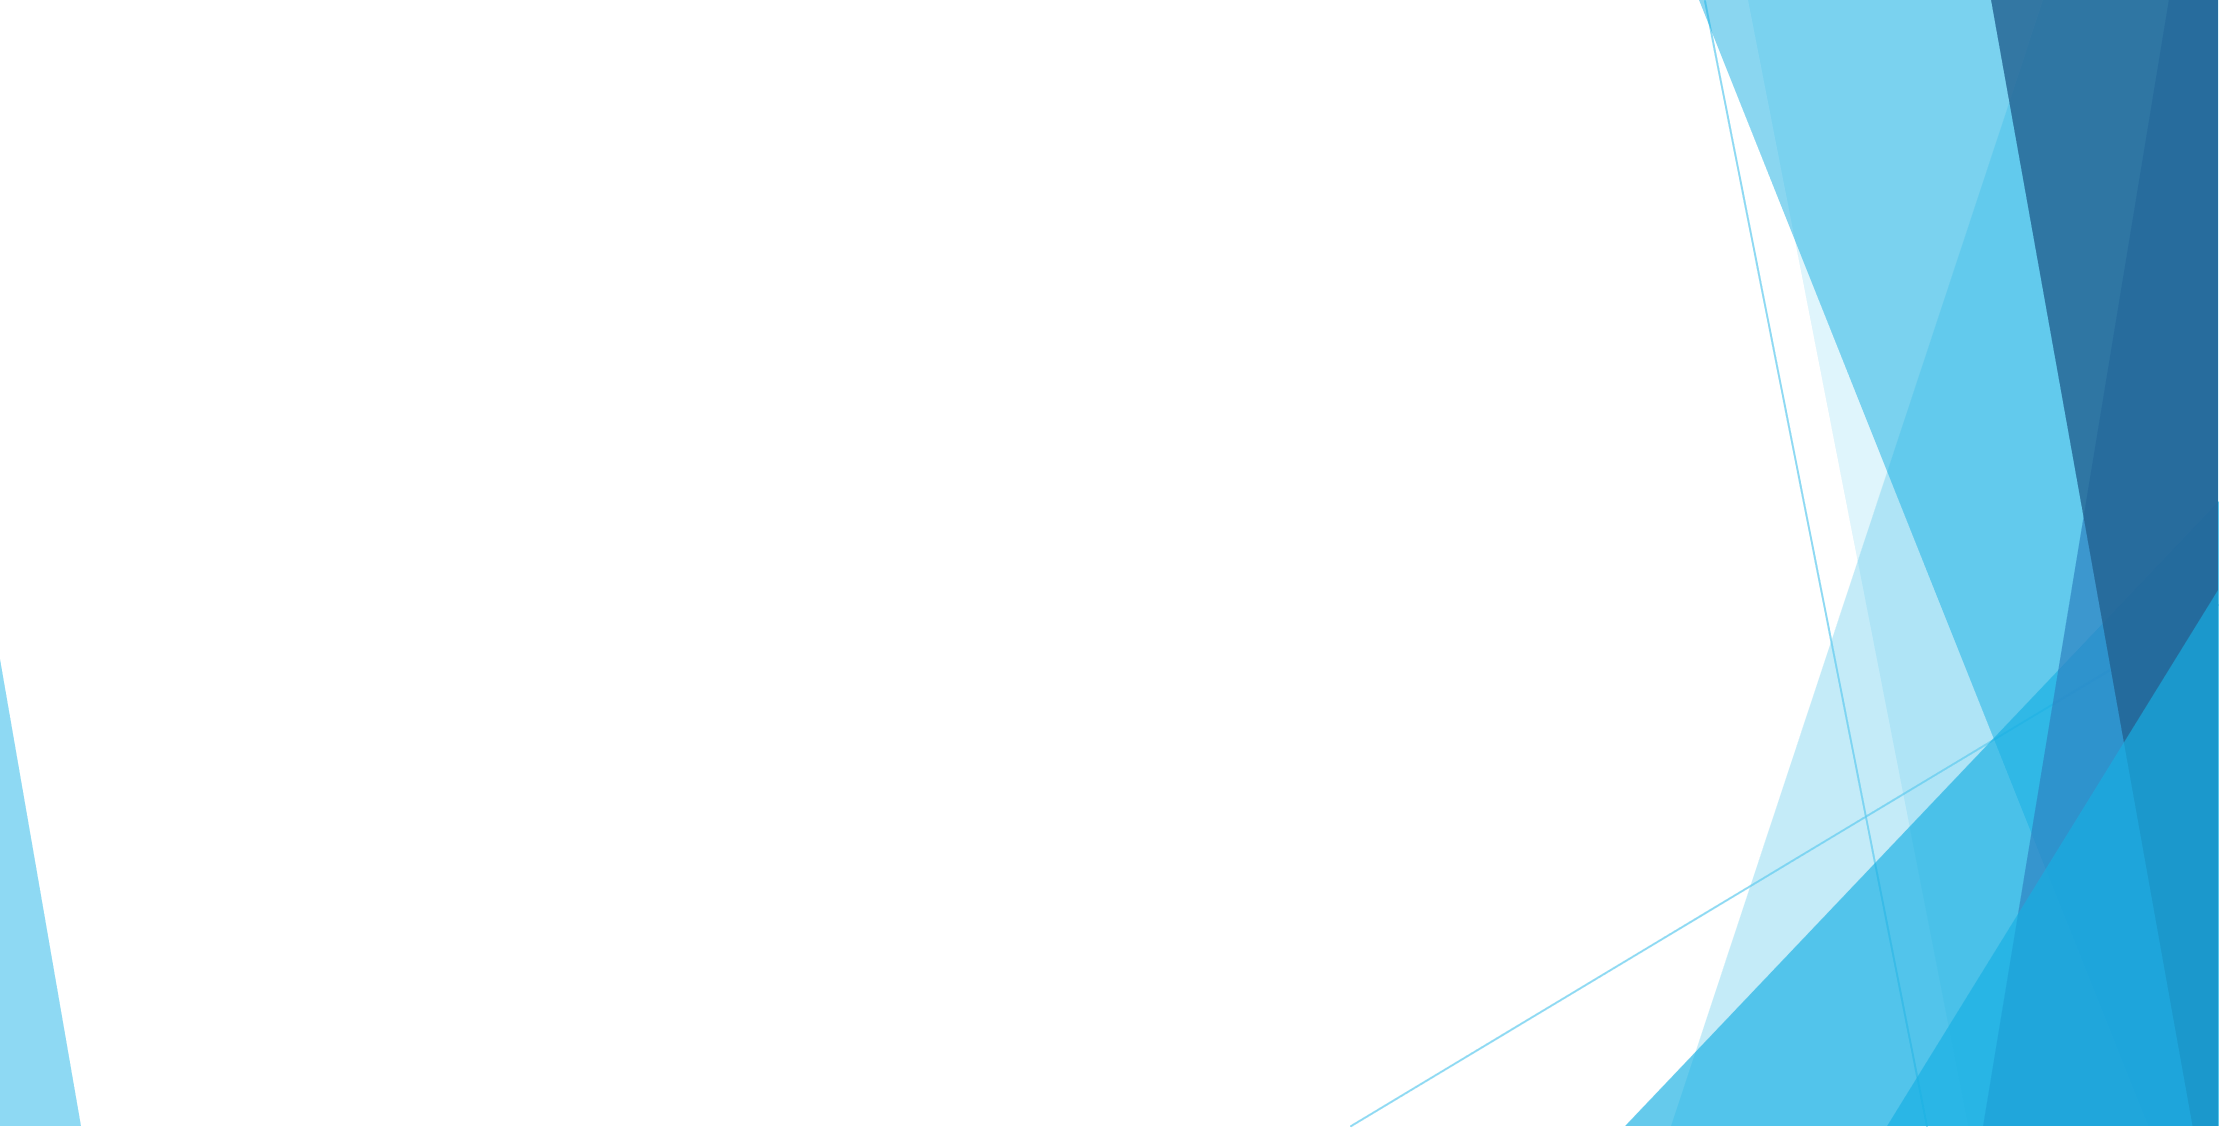
\includegraphics[width=\linewidth]{Kapitel/Kap01/test.png}
	\begin{center}
		
	
		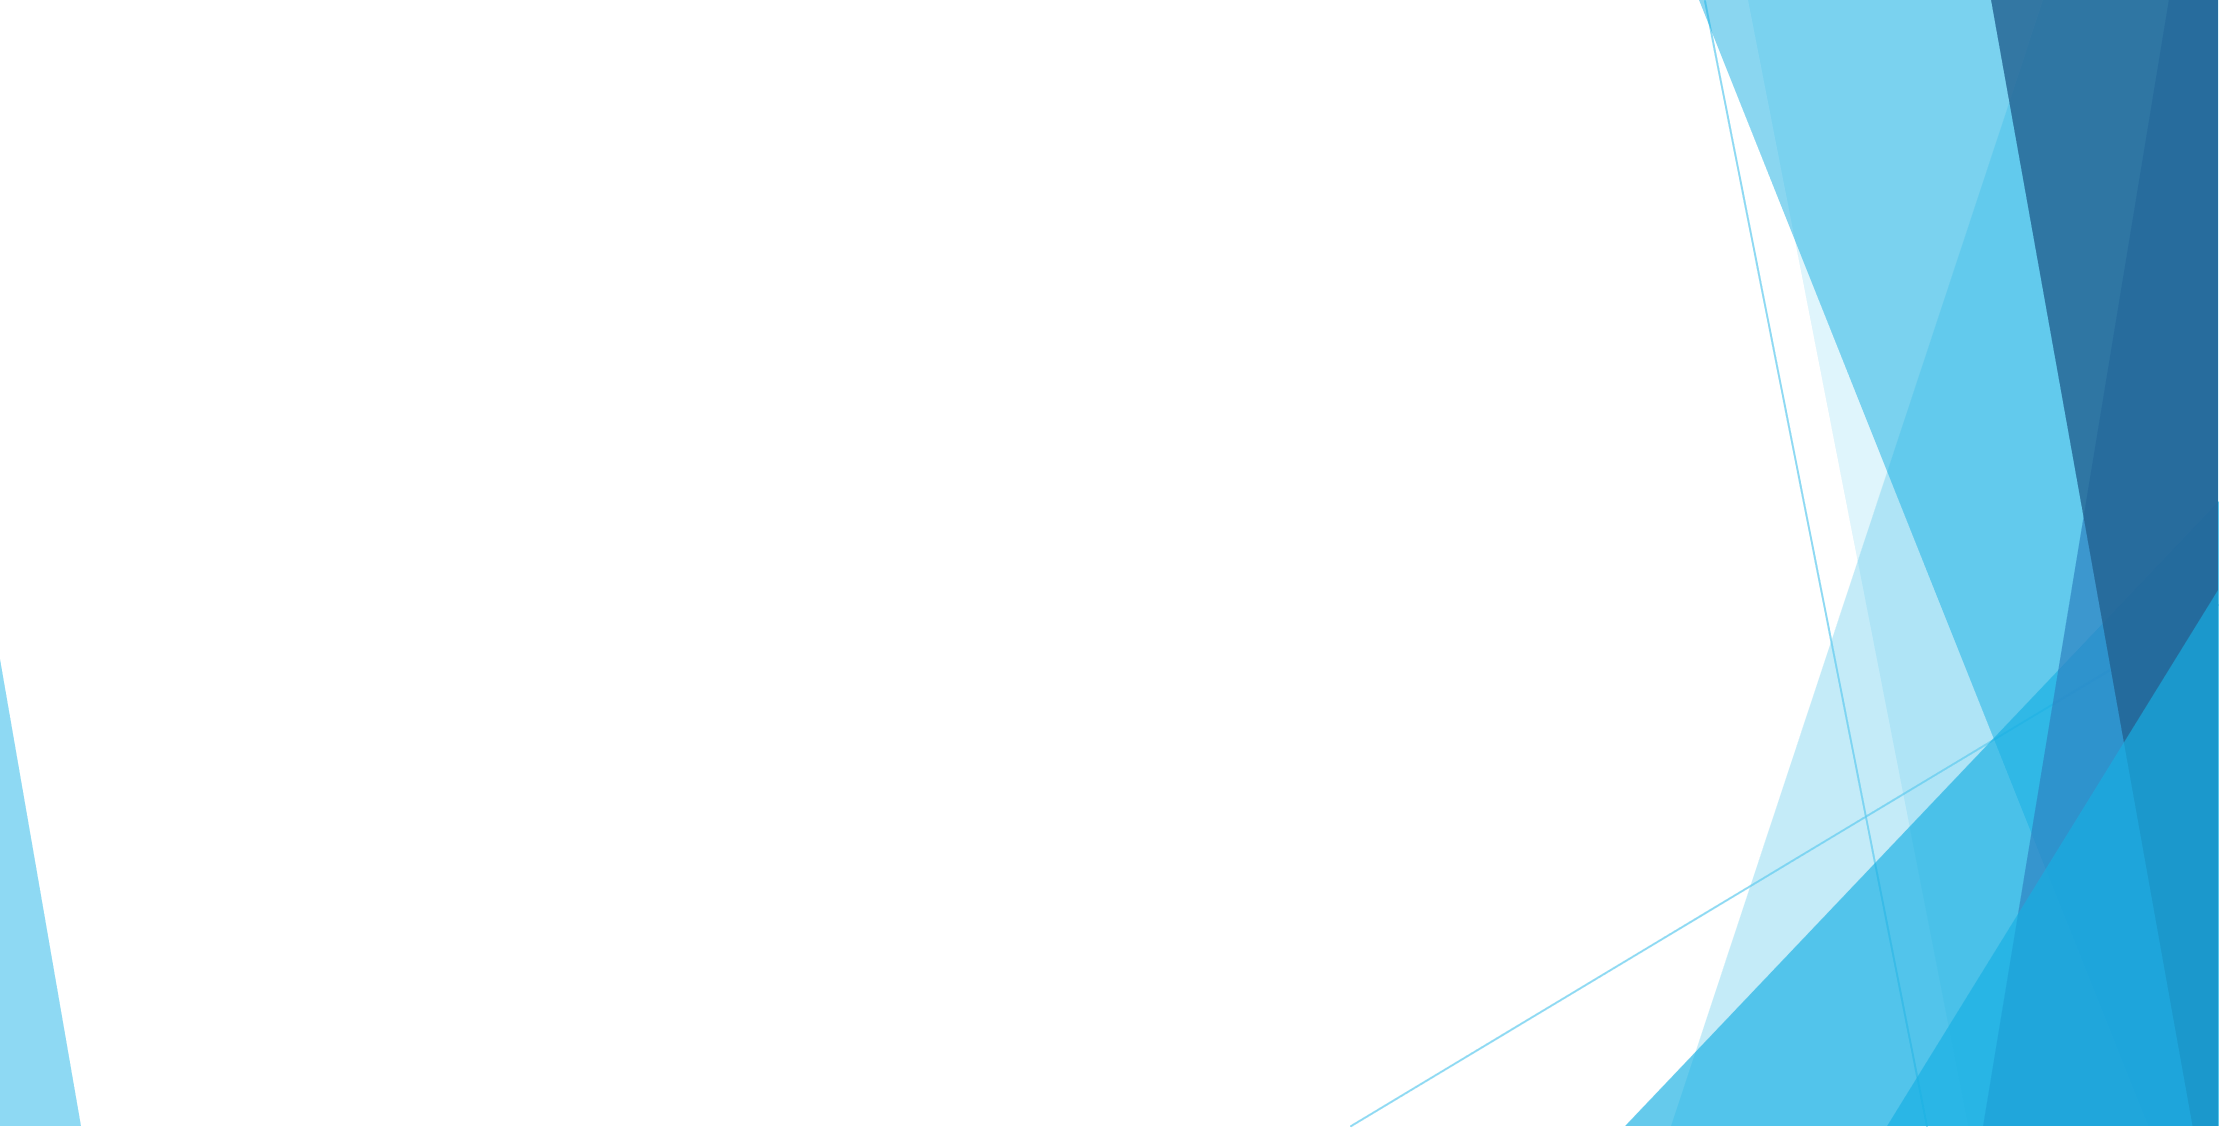
\includegraphics[width=0.4\linewidth]{Kapitel/Kap01/test.png}
	\end{center}


\begin{tabular}{|l|r|}
	\hline
	\textbf{Hello} & World\\
	\hline
	Hello & Martin\\
	\hline
\end{tabular}
\todo{Hello WOlrd}

\subsection{Verteilungsfunktion}
\subsubsection{Fermiverteilung}


Definition der Fermi-Energie
Lage des Fermi-Niveaus (intrinsisch vs. dotiert)
Effektive Zustandsdichten
Ladungsträger im Halbleiter
Massenwirkungsgesetz
Neutralitätsbedingung
Intrinsische Ladungsträgerkonzentration
Bezeichnung von dotierten Halbleitern
Majoritäten und Minoritäten
Ladungsträgerbewegung
Driftstrom, Sättigung usw.
Diffusionsstrom
Temperaturspannung
Leitfähigkeit von Halbleitern
p- und n-Typ, Temperaturabhängigkeit usw.
Definitionen von Dotierniveaus


% geometry package --> Seitenränder einstellen